\documentclass[11pt]{article} 

\usepackage{graphicx}

%%% Margenes
	\usepackage[a4paper, margin=2cm]{geometry}
	\addtolength{\topmargin}{-0.4cm}
	
%%% traduce elementos al castellano, eg "figura" en lugar de "figure"
	\usepackage[spanish]{babel} 
	
%%% 1,5 espacios de interlineado
	\renewcommand{\baselinestretch}{1.5} 

%%% colores personalizados 
	\usepackage{xcolor}
		\definecolor{RojoNebrija}{RGB}{194,0,47}
		\definecolor{GrisNebrija1}{RGB}{127,127,127}
		\definecolor{GrisNebrija2}{RGB}{166,166,166}
		\definecolor{GrisNebrija3}{RGB}{191,191,191}
		
		
%%%\renewcommand{\cftsecleader}{\cftdotfill{\cftdotsep}} % puntos separando las secciones del indice
	\setcounter{tocdepth}{2}



	
%%% cambia el color y estilo de las secciones
	\usepackage{titlesec}
		\titleformat{\section} %a rojo y subrallado
			{\color{RojoNebrija}\normalfont\Large\bfseries}
			{\thesection}{1em}{}[{\titlerule[0.5pt]}]

		\titleformat{\subsubsection} % a gris, sin numero, e indentado
			{\color{GrisNebrija1}\large}
			{}{2em}{}
			
			
%%% fin de pagina personalizado
	\usepackage{fancyhdr}
		\pagestyle{fancy}
		\futurelet\TMPfootrule\def\footrule{{\color{GrisNebrija2}\TMPfootrule}}
		\renewcommand{\footrulewidth}{0.1pt}% default is 0pt
		\fancyfoot[L]{Departamento de Ingeniería Informática – Memoria Prácticas en Empresa \ \ \ \ \thepage}
		%\fancyfoot[C]{\thepage} % numero de pagina en el centro
		%\fancyfoot[R]{\today} % fecha a la derecha
		
		%quita la cabecera
		\renewcommand{\headrulewidth}{0pt} 
		\fancyhead{}
		
		\cfoot{} % quita el numero de pagina por defecto, el del centro, dejando el manual
	

\begin{document}
	\begin{titlepage}
		{\color{white}{.}}
		\linebreak
		\linebreak
		
		\centering
		\resizebox{.8\linewidth}{!}{%
			
\includegraphics{../iconos/nebrija/antonio.pdf}
		}
		\linebreak
		\vspace{3cm}
		
		{\LARGE\textbf{\color{RojoNebrija}DESARROLLO DE UNA APLICACIÓN WEB Y ESTUDIO DE HERRAMIENTAS PARA EL DESPLIEGUE DE SU INFRAESTRUCTURA}\par}
		\vspace{2cm}
		
		{\Large \textbf{\color{black}UNIVERSIDAD NEBRIJA \\ GRADO EN INGENIERÍA INFORMÁTICA \\ MEMORIA PRÁCTICAS EN EMPRESA}\par}
		\vspace{2cm}
		

		{\Large \textbf{ Óscar Salvador Sotoca\\ Enero/2023}\par}
		\vspace{2cm}

		{\Large \textbf{Tutor académico: Carlos Castellanos Manzaneque}\par}
		\vspace{2cm}
						
		%\resizebox{.4\linewidth}{!}{%
		%	
\includegraphics{./nebrija.pdf}
		%}
		
		%\resizebox{.4\linewidth}{!}{%
		%	
\includegraphics{./global.pdf}
		%}
		
		
	%\maketitle
	\end{titlepage}


\tableofcontents

\clearpage
\listoffigures

\begin{flushleft}

\clearpage
\section{Experiencia en empresa}
tbc
\linebreak

	\subsection{Introduccion, mis responsabilidades}
	\subsection{Onboarding}
	\subsection{Organigrama}








 


\clearpage
\section{Proyecto}
El estado del arte para el aprovisionado de infraestructura es contratarla, de manera flexible, a un proveedor cloud. En particular, aún más recientemente se ha apostado por la descripción de la infraestructura a contratar, en lenguajes declarativos y de programación general.

Este nuevo paradigma, Infraestructura como Código, ofrece replicabilidad y  reutilización, pero en particular permite afrontar el mantenimiento de esta con técnicas de desarrollo convencionales como el control de versiones.
	\linebreak

En este proyecto exploraré dos de las soluciones de Infraestructura como Código más competentes y populares: Terraform y Ansible (en particular Ansible Playbooks). Las usaré para contratar en un proveedor cloud los recursos necesarios para un sistema full stack desarrollado específicamente para este proyecto.
	\linebreak

Después de explicar cómo funciona cada una y ponerlas en uso, compararé sus características y contrastaré sus ventajas.


	\subsection{Antecedentes}
		Este no es un proyecto original, la aplicación que quiero implementar debería ser una maqueta representativa de los elementos y comportamientos del sistema moderno medio del mercado. El valor añadido será la explicación del de esta, y la comparación entre herramientas comerciales.

		
	\subsection{Estudio del problema}
		He descompuesto el problema en tres fases de trabajo:
		\begin{enumerate}
			%\addtolength{\itemindent}{0.80cm}
			\itemsep0em 
			\item Programación de componentes lógicos (front-end, middleware) en local, usando Docker para prototipar e iterar rápido
			\item Creación manual de los recursos y migración a la nube
			\item Descripción de la infraestructura como código con ambas herramientas y comparación de ellas
		\end{enumerate}
		
	\subsection{Objetivos}
		\begin{enumerate}
			%\addtolength{\itemindent}{0.80cm}
			\itemsep0em 
			\item Implementar un sistema full-stack representativo de la arquitectura que se podría encontrar en una aplicación comercial
				\begin{enumerate}
					%\addtolength{\itemindent}{0.80cm}
					\itemsep0em 
					\item Servidor de estáticos, con el Front-end
					\item Servidor de contenido, con imágenes que se usen en el Front-end
					\item Middleware de una sola capa, API con GraphQL
						\begin{itemize}
							%\addtolength{\itemindent}{0.80cm}
							\itemsep0em 
							\item Base de datos para tokens de sesión
						\end{itemize}
					\item Back-end: Persistencia usando una base de datos MongoDB
				\end{enumerate}
			\item Desarrollar el código necesario para contratar la infraestructura necesaria en Terraform y Ansible, y compararlos
		\end{enumerate}















\clearpage
\section{Aplicación}
El caso de uso que propongo es una aplicación web. Basada en los contenidos de la asignatura de desarrollo front-end, similar a las prácticas cuatro (full stack, CRUD en REST) y cinco (solo front-end, GraphQL), y un ejercicio de clase (full stack, GraphQL con tokens de verificación). todas en React. 
\linebreak

La página permite ver “posts”, compuestos por: el nombre del usuario que lo ha publicado, un comentario, y una imagen. Los comentarios pueden verse sin iniciar sesión (login). Un usuario sin identificarse puede iniciar sesión o registrarse. La segunda crea un usuario y después dispara el login automáticamente. Un usuario identificado puede: Hacer posts, lo que implica subir una imagen y un comentario; borrar los comentarios de los que sea autor; y hacer cerrar sesión (logout). 
\linebreak 

Las diferencias principales frente a las anteriores son: el uso de una base de datos Redis, para guardar los tokens solo en memoria; el almacenamiento de imágenes, usando un S3; y un reverse proxy para solucionar el problema que presenta la seguridad contra CORS. 
\linebreak

	\begin{figure}[htb]
		\centering
		\resizebox{.8\linewidth}{!}{%
			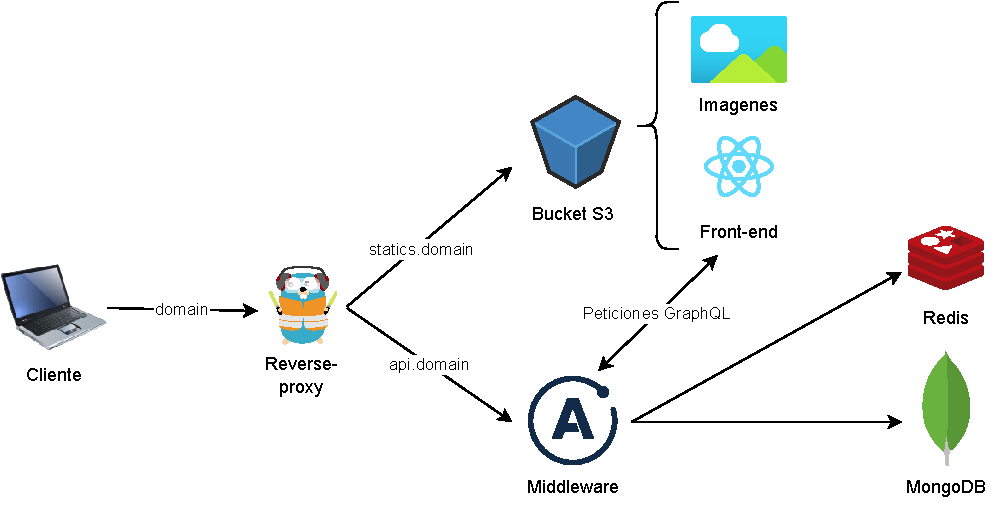
\includegraphics{../drawio/general.drawio-1.pdf}
		}
		\caption{Diseño a alto nivel (O. Salvador 2022)}
	\end{figure}

Según el proveedor cloud, algunos de los elementos se pueden contratar como Software as a Service, pagando por el uso en lugar de la maquina sobre la que correr el componente.  
\linebreak
 

Hasta la entrega parcial estoy en la primera fase del problema, desarrollando en local con Docker. Todas las siguientes llamadas están implementadas, pero la interacción para subir una imagen al s3 está a medias. Para este hito, solo he conseguido subir la imagen a un s3 público. Tendré que solucionar el manejo de permisos para que, aunque la lectura sea publica, la escritura dependa de credenciales. 


	\subsection{Inicio de sesión}
		El cliente front-end estará preparado en el S3. El cliente entra al dominio, el proxy dirige la petición inicial hacia los estáticos, y le sirve el JavaScript del front-end.
		\linebreak
		
		Desde el cliente se piden los ``posts''. Estos comentarios están guardados en mongo. Cada post contiene una dirección a su imagen correspondiente. Esta esta guardada en el S3, y solo referenciada en el post. Una vez el cliente tiene la lista de posts, para cada uno, pide su archivo correspondiente. Esta operación no necesita login, es pública. El bucket tendrá permisos de lectura públicos, pero de escritura restringidos.  
		\linebreak
		
			\begin{figure}[htb]
				\centering
				\resizebox{.8\linewidth}{!}{%
					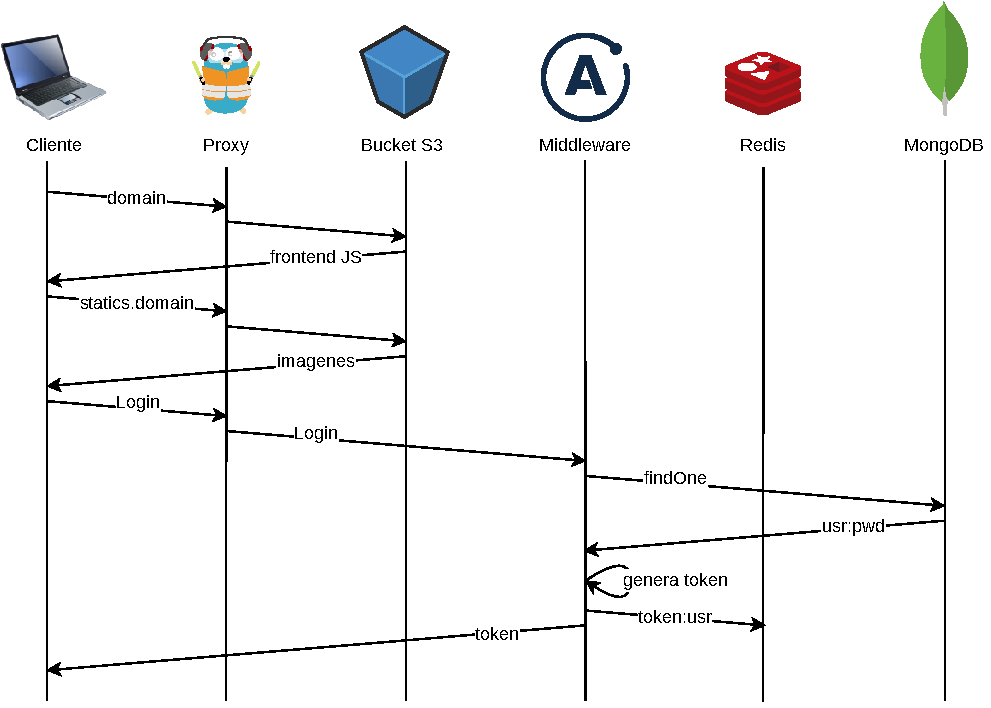
\includegraphics{../drawio/login.drawio.pdf}
				}
				\caption{Paso de mensajes durante login (O. Salvador 2022)}
			\end{figure}	
	
		Con el cliente renderizado, el usuario puede hacer clic en el único botón, login. Desde aquí, puede iniciar sesión si ya se tiene usuario, o crear uno nuevo. Ninguna de estas dos peticiones necesita autorización.  
		\linebreak
		

		Crear usuario pide un nombre y contraseña. la última se tiene que escribir dos veces y debe tener caracteres variados, por seguridad. Si ya hay un usuario con ese nombre, el back-end rechazara la petición. En el caso contrario, la operación se completa y de vuelta en el cliente se dispara un login con las credenciales del usuario recién creado. 
		\linebreak
		
		
	\clearpage
		El usuario puede hacer login en el cliente, enviando su usuario y contraseña, por ahora en claro (mi objetivo es pasarlo por TLS, lo hare cuando la esté bien y tenga certificados). La petición es reconocida en el proxy y reenviada al middleware. Por la escala de la práctica y su longevidad, he hecho un middleware unificado, en lugar de separarlo en front (más expuesto, y sin estado) y back (con sesión). 
		\linebreak
		
			\begin{figure}[htb]
				\centering
				\resizebox{.8\linewidth}{!}{%
					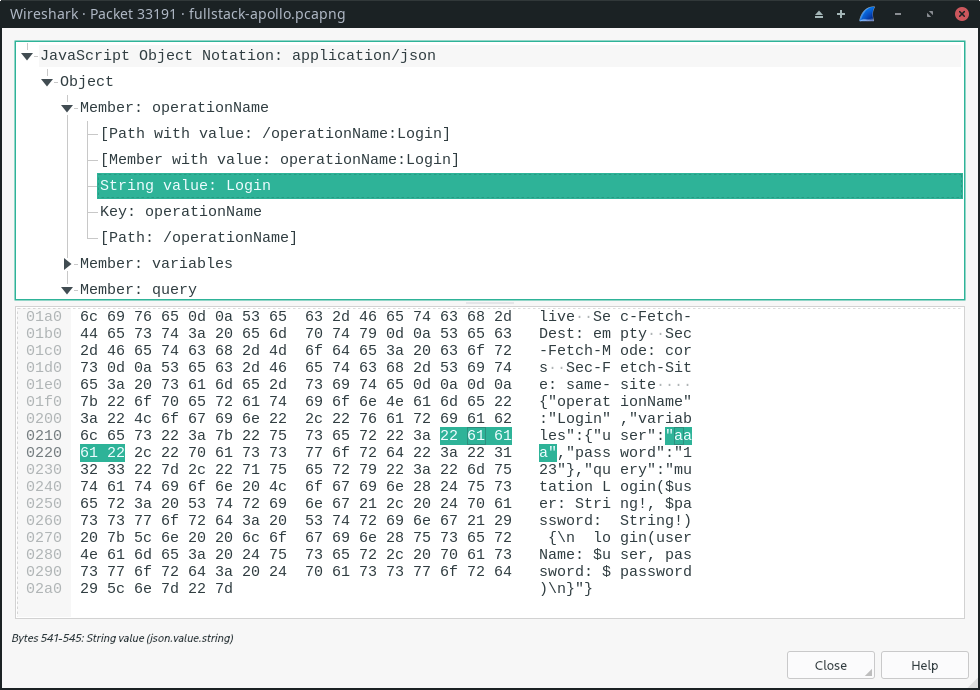
\includegraphics{../capturas/wireshark-login.png}
				}
				\caption{Inspección de los mensajes durante login usando Wireshark (O. Salvador 2022)}
			\end{figure}	

		Desde el middleware, se hace una petición a Mongo y comprueban las credenciales en la colección ``users''. Si son correctos, se genera un token, y se añade este y el nombre de usuario como entrada en Redis. finalmente, se devuelve al cliente el token del usuario, donde es guardado como una cookie el token tiene una caducidad de una hora. 
		\linebreak
		
		Inmediatamente después de hacer login, se vuelve a preguntar al middleware los posts, enviando el token. Ahí, este es resuelto al nombre de usuario, y comparado con el de los posts, y se levanta un flag en todos los posts que sean del usuario haciendo la petición.  
		\linebreak
 
		El resto de las peticiones al middleware requieren del cliente el uso de la cabecera "Authorization", con un token valido, que se comprueba con cada una. La lista es recibida por el cliente y se vuelve a pintar. Los posts del usuario reciben un botón para borrarlos. Si estos son pulsados, se envía una petición con el \_id en la colección de mongo, con el que se identifican en el back y borrados de la colección. 
		\linebreak
		
		
	\subsection{CRUD de contenido de usuarios}
		Partiendo de un usuario autenticado, cuando el usuario selecciona el botón “Send” en el Modal post, dispara la petición GraphQL “addPost”, que recibe el comentario escrito. El middleware, soluciona el token del usuario a su nombre. Además, con los credenciales del bucket, que nunca salen del middleware, se genera una URL firmada en la que el cliente puede subir una imagen. Esta es añadida junto a los otros detalles como una nueva entrada a la colección de Mongo. La URL es devuelta al cliente, y la imagen se sube desde este. 
		\linebreak
		
			\begin{figure}[htb]
				\centering
				\resizebox{.8\linewidth}{!}{%
					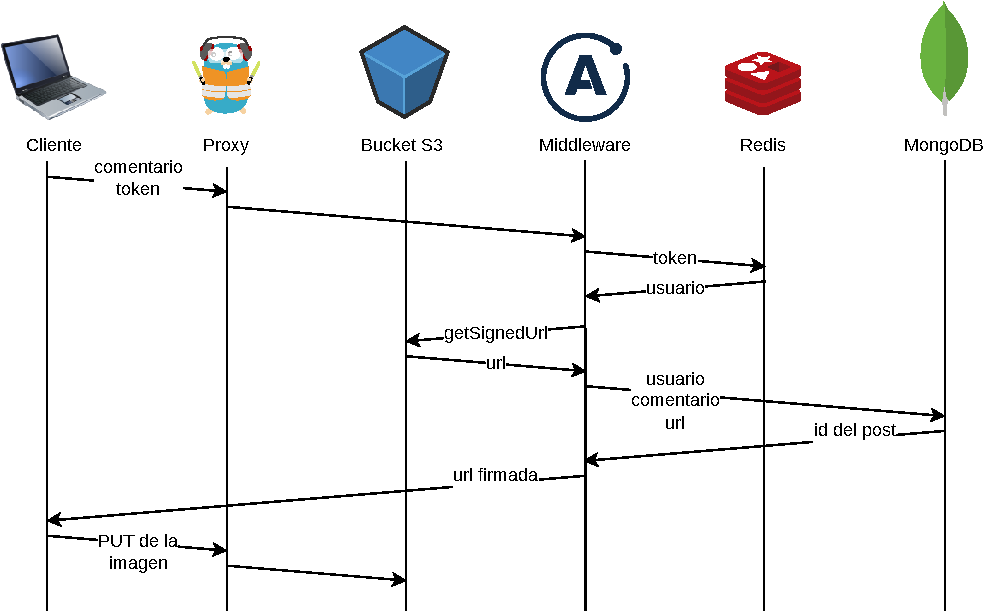
\includegraphics{../drawio/crud.pdf}
				}
				\caption{Paso de mensajes para añadir post (O. Salvador 2022)}
			\end{figure}	
			
		Este método permite mantener los credenciales seguros, no dejándolos pasar por el cliente en ningún momento. Al mismo tiempo, permite ahorrar ancho de banda, subiendo la imagen directamente al bucket, en lugar de hacerla pasar primero al middleware. 
		\linebreak
		
\section{Infraestructura}
tbc

\section{Comparación}
tbc

\section{Conclusión}




\end{flushleft}
\end{document}
